\documentclass{extbook}[14pt]
\usepackage{multicol, enumerate, enumitem, hyperref, color, soul, setspace, parskip, fancyhdr, amssymb, amsthm, amsmath, bbm, latexsym, units, mathtools}
\everymath{\displaystyle}
\usepackage[headsep=0.5cm,headheight=0cm, left=1 in,right= 1 in,top= 1 in,bottom= 1 in]{geometry}
\usepackage{dashrule}  % Package to use the command below to create lines between items
\newcommand{\litem}[1]{\item #1

\rule{\textwidth}{0.4pt}}
\pagestyle{fancy}
\lhead{}
\chead{Answer Key for Progress Quiz 10 Version B}
\rhead{}
\lfoot{6232-9639}
\cfoot{}
\rfoot{Fall 2020}
\begin{document}
\textbf{This key should allow you to understand why you choose the option you did (beyond just getting a question right or wrong). \href{https://xronos.clas.ufl.edu/mac1105spring2020/courseDescriptionAndMisc/Exams/LearningFromResults}{More instructions on how to use this key can be found here}.}

\textbf{If you have a suggestion to make the keys better, \href{https://forms.gle/CZkbZmPbC9XALEE88}{please fill out the short survey here}.}

\textit{Note: This key is auto-generated and may contain issues and/or errors. The keys are reviewed after each exam to ensure grading is done accurately. If there are issues (like duplicate options), they are noted in the offline gradebook. The keys are a work-in-progress to give students as many resources to improve as possible.}

\rule{\textwidth}{0.4pt}

\begin{enumerate}\litem{
Describe the end behavior of the polynomial below.
\[ f(x) = -6(x + 5)^{2}(x - 5)^{5}(x + 6)^{5}(x - 6)^{5} \]

The solution is the graph below, which is option A.
\begin{center}
    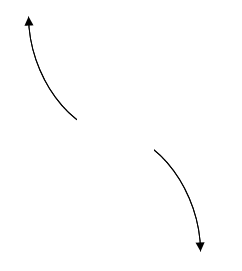
\includegraphics[width=0.3\textwidth]{../Figures/polyEndBehaviorAB.png}
\end{center}\begin{enumerate}[label=\Alph*.]
\begin{multicols}{2}
\item 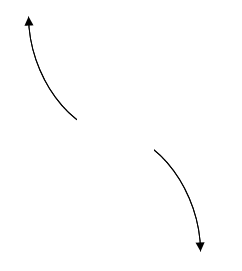
\includegraphics[width = 0.3\textwidth]{../Figures/polyEndBehaviorAB.png}
\item 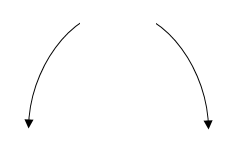
\includegraphics[width = 0.3\textwidth]{../Figures/polyEndBehaviorBB.png}
\item 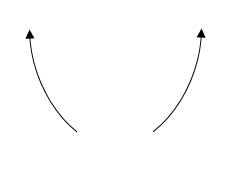
\includegraphics[width = 0.3\textwidth]{../Figures/polyEndBehaviorCB.png}
\item 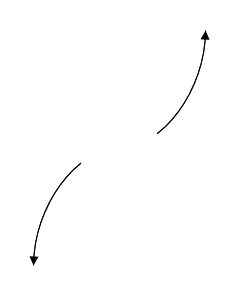
\includegraphics[width = 0.3\textwidth]{../Figures/polyEndBehaviorDB.png}
\end{multicols}\item None of the above.\end{enumerate}
\textbf{General Comment:} Remember that end behavior is determined by the leading coefficient AND whether the \textbf{sum} of the multiplicities is positive or negative.
}
\litem{
Construct the lowest-degree polynomial given the zeros below. Then, choose the intervals that contain the coefficients of the polynomial in the form $x^3+bx^2+cx+d$.
\[ 3 - 5 i \text{ and } -1 \]

The solution is \( x^{3} -5 x^{2} +28 x + 34 \), which is option C.\begin{enumerate}[label=\Alph*.]
\item \( b \in [0, 3.1], c \in [-11, 2], \text{ and } d \in [-8, 1] \)

$x^{3} + x^{2} -2 x -3$, which corresponds to multiplying out $(x -3)(x + 1)$.
\item \( b \in [1.1, 5.6], c \in [20, 29], \text{ and } d \in [-35, -31] \)

$x^{3} +5 x^{2} +28 x -34$, which corresponds to multiplying out $(x-(3 - 5 i))(x-(3 + 5 i))(x -1)$.
\item \( b \in [-5.2, -3], c \in [20, 29], \text{ and } d \in [31, 38] \)

* $x^{3} -5 x^{2} +28 x + 34$, which is the correct option.
\item \( b \in [0, 3.1], c \in [1, 9], \text{ and } d \in [0, 8] \)

$x^{3} + x^{2} +6 x + 5$, which corresponds to multiplying out $(x + 5)(x + 1)$.
\item \( \text{None of the above.} \)

This corresponds to making an unanticipated error or not understanding how to use nonreal complex numbers to create the lowest-degree polynomial. If you chose this and are not sure what you did wrong, please contact the coordinator for help.
\end{enumerate}

\textbf{General Comment:} Remember that the conjugate of $a+bi$ is $a-bi$. Since these zeros always come in pairs, we need to multiply out $(x-(3 - 5 i))(x-(3 + 5 i))(x-(-1))$.
}
\litem{
Describe the zero behavior of the zero $x = 9$ of the polynomial below.
\[ f(x) = 8(x + 9)^{5}(x - 9)^{10}(x - 8)^{8}(x + 8)^{12} \]

The solution is the graph below, which is option C.
\begin{center}
    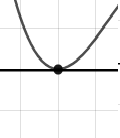
\includegraphics[width=0.3\textwidth]{../Figures/polyZeroBehaviorCopyCB.png}
\end{center}\begin{enumerate}[label=\Alph*.]
\begin{multicols}{2}
\item 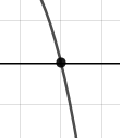
\includegraphics[width = 0.3\textwidth]{../Figures/polyZeroBehaviorCopyAB.png}
\item 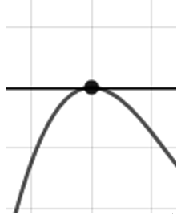
\includegraphics[width = 0.3\textwidth]{../Figures/polyZeroBehaviorCopyBB.png}
\item 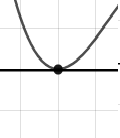
\includegraphics[width = 0.3\textwidth]{../Figures/polyZeroBehaviorCopyCB.png}
\item 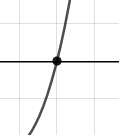
\includegraphics[width = 0.3\textwidth]{../Figures/polyZeroBehaviorCopyDB.png}
\end{multicols}\item None of the above.\end{enumerate}
\textbf{General Comment:} You will need to sketch the entire graph, then zoom in on the zero the question asks about.
}
\litem{
Construct the lowest-degree polynomial given the zeros below. Then, choose the intervals that contain the coefficients of the polynomial in the form $ax^3+bx^2+cx+d$.
\[ 1, \frac{-3}{4}, \text{ and } \frac{-5}{3} \]

The solution is \( 12x^{3} +17 x^{2} -14 x -15 \), which is option D.\begin{enumerate}[label=\Alph*.]
\item \( a \in [12, 19], b \in [14.9, 17.6], c \in [-25, -7], \text{ and } d \in [10, 23] \)

$12x^{3} +17 x^{2} -14 x + 15$, which corresponds to multiplying everything correctly except the constant term.
\item \( a \in [12, 19], b \in [22.9, 25], c \in [-9, -3], \text{ and } d \in [-15, -12] \)

$12x^{3} +23 x^{2} -4 x -15$, which corresponds to multiplying out $(x + 1)(4x -3)(3x + 5)$.
\item \( a \in [12, 19], b \in [-19.1, -15.4], c \in [-25, -7], \text{ and } d \in [10, 23] \)

$12x^{3} -17 x^{2} -14 x + 15$, which corresponds to multiplying out $(x + 1)(4x -3)(3x -5)$.
\item \( a \in [12, 19], b \in [14.9, 17.6], c \in [-25, -7], \text{ and } d \in [-15, -12] \)

* $12x^{3} +17 x^{2} -14 x -15$, which is the correct option.
\item \( a \in [12, 19], b \in [40.2, 44], c \in [38, 47], \text{ and } d \in [10, 23] \)

$12x^{3} +41 x^{2} +44 x + 15$, which corresponds to multiplying out $(x + 1)(4x + 3)(3x + 5)$.
\end{enumerate}

\textbf{General Comment:} To construct the lowest-degree polynomial, you want to multiply out $(x -1)(4x + 3)(3x + 5)$
}
\litem{
Which of the following equations \textit{could} be of the graph presented below?

\begin{center}
    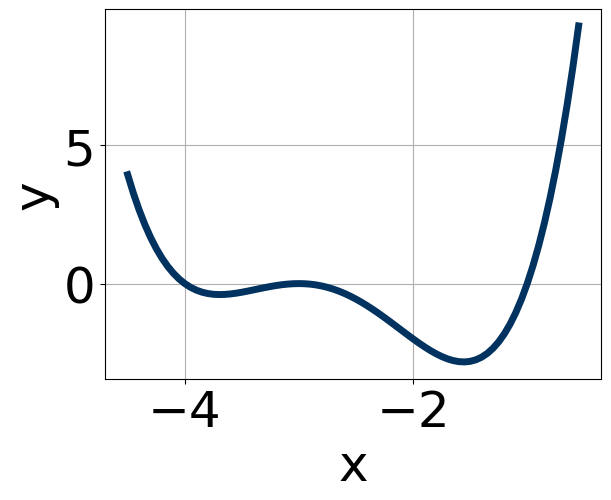
\includegraphics[width=0.5\textwidth]{../Figures/polyGraphToFunctionB.png}
\end{center}




The solution is \( 2(x + 3)^{8} (x + 1)^{7} (x + 4)^{5} \), which is option C.\begin{enumerate}[label=\Alph*.]
\item \( 16(x + 3)^{5} (x + 1)^{6} (x + 4)^{11} \)

The factor $-3$ should have an even power and the factor $-1$ should have an odd power.
\item \( 19(x + 3)^{6} (x + 1)^{10} (x + 4)^{7} \)

The factor $(x + 1)$ should have an odd power.
\item \( 2(x + 3)^{8} (x + 1)^{7} (x + 4)^{5} \)

* This is the correct option.
\item \( -3(x + 3)^{8} (x + 1)^{9} (x + 4)^{10} \)

The factor $(x + 4)$ should have an odd power and the leading coefficient should be the opposite sign.
\item \( -20(x + 3)^{4} (x + 1)^{11} (x + 4)^{9} \)

This corresponds to the leading coefficient being the opposite value than it should be.
\end{enumerate}

\textbf{General Comment:} General Comments: Draw the x-axis to determine which zeros are touching (and so have even multiplicity) or cross (and have odd multiplicity).
}
\litem{
Describe the zero behavior of the zero $x = -6$ of the polynomial below.
\[ f(x) = 5(x - 6)^{5}(x + 6)^{8}(x - 9)^{9}(x + 9)^{11} \]

The solution is the graph below, which is option C.
\begin{center}
    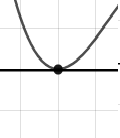
\includegraphics[width=0.3\textwidth]{../Figures/polyZeroBehaviorCB.png}
\end{center}\begin{enumerate}[label=\Alph*.]
\begin{multicols}{2}
\item 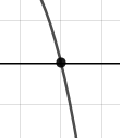
\includegraphics[width = 0.3\textwidth]{../Figures/polyZeroBehaviorAB.png}
\item 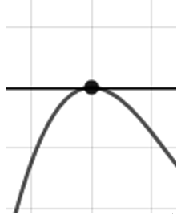
\includegraphics[width = 0.3\textwidth]{../Figures/polyZeroBehaviorBB.png}
\item 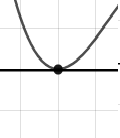
\includegraphics[width = 0.3\textwidth]{../Figures/polyZeroBehaviorCB.png}
\item 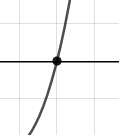
\includegraphics[width = 0.3\textwidth]{../Figures/polyZeroBehaviorDB.png}
\end{multicols}\item None of the above.\end{enumerate}
\textbf{General Comment:} You will need to sketch the entire graph, then zoom in on the zero the question asks about.
}
\litem{
Describe the end behavior of the polynomial below.
\[ f(x) = 2(x + 2)^{2}(x - 2)^{3}(x + 3)^{3}(x - 3)^{5} \]

The solution is the graph below, which is option D.
\begin{center}
    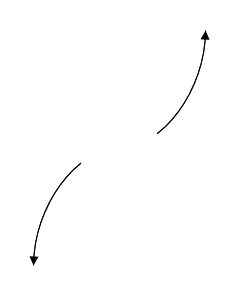
\includegraphics[width=0.3\textwidth]{../Figures/polyEndBehaviorCopyDB.png}
\end{center}\begin{enumerate}[label=\Alph*.]
\begin{multicols}{2}
\item 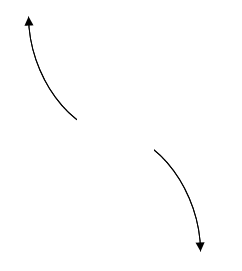
\includegraphics[width = 0.3\textwidth]{../Figures/polyEndBehaviorCopyAB.png}
\item 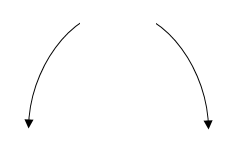
\includegraphics[width = 0.3\textwidth]{../Figures/polyEndBehaviorCopyBB.png}
\item 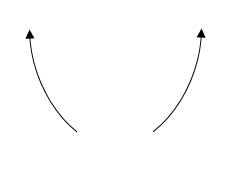
\includegraphics[width = 0.3\textwidth]{../Figures/polyEndBehaviorCopyCB.png}
\item 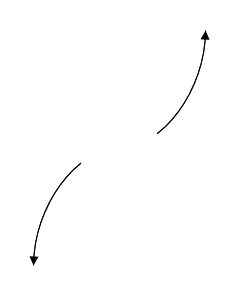
\includegraphics[width = 0.3\textwidth]{../Figures/polyEndBehaviorCopyDB.png}
\end{multicols}\item None of the above.\end{enumerate}
\textbf{General Comment:} Remember that end behavior is determined by the leading coefficient AND whether the \textbf{sum} of the multiplicities is positive or negative.
}
\litem{
Construct the lowest-degree polynomial given the zeros below. Then, choose the intervals that contain the coefficients of the polynomial in the form $x^3+bx^2+cx+d$.
\[ 4 - 3 i \text{ and } 1 \]

The solution is \( x^{3} -9 x^{2} +33 x -25 \), which is option B.\begin{enumerate}[label=\Alph*.]
\item \( b \in [-2, 6], c \in [-1, 13], \text{ and } d \in [-5, -1] \)

$x^{3} + x^{2} +2 x -3$, which corresponds to multiplying out $(x + 3)(x -1)$.
\item \( b \in [-13, -8], c \in [31, 36], \text{ and } d \in [-26, -23] \)

* $x^{3} -9 x^{2} +33 x -25$, which is the correct option.
\item \( b \in [8, 11], c \in [31, 36], \text{ and } d \in [25, 31] \)

$x^{3} +9 x^{2} +33 x + 25$, which corresponds to multiplying out $(x-(4 - 3 i))(x-(4 + 3 i))(x + 1)$.
\item \( b \in [-2, 6], c \in [-10, -1], \text{ and } d \in [0, 5] \)

$x^{3} + x^{2} -5 x + 4$, which corresponds to multiplying out $(x -4)(x -1)$.
\item \( \text{None of the above.} \)

This corresponds to making an unanticipated error or not understanding how to use nonreal complex numbers to create the lowest-degree polynomial. If you chose this and are not sure what you did wrong, please contact the coordinator for help.
\end{enumerate}

\textbf{General Comment:} Remember that the conjugate of $a+bi$ is $a-bi$. Since these zeros always come in pairs, we need to multiply out $(x-(4 - 3 i))(x-(4 + 3 i))(x-(1))$.
}
\litem{
Which of the following equations \textit{could} be of the graph presented below?

\begin{center}
    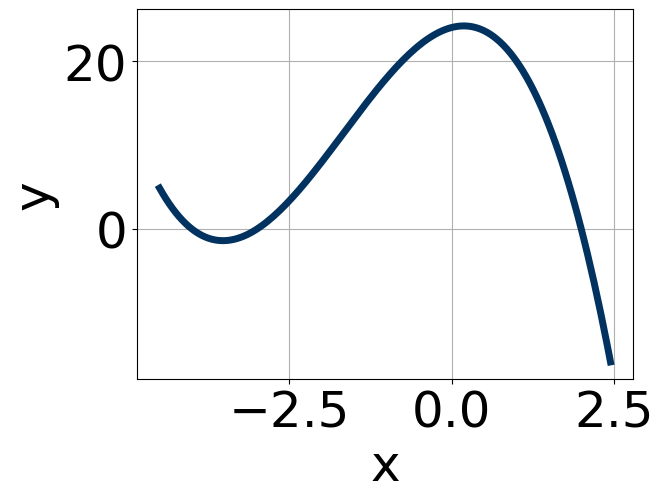
\includegraphics[width=0.5\textwidth]{../Figures/polyGraphToFunctionCopyB.png}
\end{center}




The solution is \( -11(x + 3)^{11} (x + 4)^{9} (x - 2)^{5} \), which is option C.\begin{enumerate}[label=\Alph*.]
\item \( -3(x + 3)^{8} (x + 4)^{6} (x - 2)^{11} \)

The factors $-3$ and $-4$ have have been odd power.
\item \( 16(x + 3)^{10} (x + 4)^{11} (x - 2)^{7} \)

The factor $(x + 3)$ should have an odd power and the leading coefficient should be the opposite sign.
\item \( -11(x + 3)^{11} (x + 4)^{9} (x - 2)^{5} \)

* This is the correct option.
\item \( 2(x + 3)^{11} (x + 4)^{11} (x - 2)^{9} \)

This corresponds to the leading coefficient being the opposite value than it should be.
\item \( -9(x + 3)^{4} (x + 4)^{7} (x - 2)^{11} \)

The factor $-3$ should have been an odd power.
\end{enumerate}

\textbf{General Comment:} General Comments: Draw the x-axis to determine which zeros are touching (and so have even multiplicity) or cross (and have odd multiplicity).
}
\litem{
Construct the lowest-degree polynomial given the zeros below. Then, choose the intervals that contain the coefficients of the polynomial in the form $ax^3+bx^2+cx+d$.
\[ 3, 4, \text{ and } \frac{-1}{2} \]

The solution is \( 2x^{3} -13 x^{2} +17 x + 12 \), which is option D.\begin{enumerate}[label=\Alph*.]
\item \( a \in [-4, 5], b \in [14, 19], c \in [26, 35], \text{ and } d \in [7, 17] \)

$2x^{3} +15 x^{2} +31 x + 12$, which corresponds to multiplying out $(x + 3)(x + 4)(2x + 1)$.
\item \( a \in [-4, 5], b \in [-21, -10], c \in [11, 26], \text{ and } d \in [-12, -10] \)

$2x^{3} -13 x^{2} +17 x -12$, which corresponds to multiplying everything correctly except the constant term.
\item \( a \in [-4, 5], b \in [-4, 10], c \in [-27, -20], \text{ and } d \in [-12, -10] \)

$2x^{3} -1 x^{2} -25 x -12$, which corresponds to multiplying out $(x + 3)(x -4)(2x + 1)$.
\item \( a \in [-4, 5], b \in [-21, -10], c \in [11, 26], \text{ and } d \in [7, 17] \)

* $2x^{3} -13 x^{2} +17 x + 12$, which is the correct option.
\item \( a \in [-4, 5], b \in [9, 14], c \in [11, 26], \text{ and } d \in [-12, -10] \)

$2x^{3} +13 x^{2} +17 x -12$, which corresponds to multiplying out $(x + 3)(x + 4)(2x -1)$.
\end{enumerate}

\textbf{General Comment:} To construct the lowest-degree polynomial, you want to multiply out $(x -3)(x -4)(2x + 1)$
}
\end{enumerate}

\end{document}